\section{Some preliminary results}

With a given probability of forming a bond between two nodes that are at a distance $r$ away from each other to be $r^{-\sigma}$, we expect the correlation function $\xi(r)$(i.e. the distribution of distances at which two nodes are bound) to follow $\sim r^{-\sigma}$. We show in the figure \ref{fig:correlationFunction} the measured average (black, solid line) correlation function and its standard deviation (black, dashed lines) after generating 1000 realizations of the connection graph using Walker's Alias algorithm to draw the bonds among the nodes. In pink, overlayed on top of the black curve, the fit of the average $\xi(r)$ is shown. We fit $\xi(r)$ to the curve $y = (a r + b) ^{-\sigma}$ and obtain a perfect overlay between the data (the average $\xi(r)$) and the fit curve.

\begin{figure}[h]
	\centering
	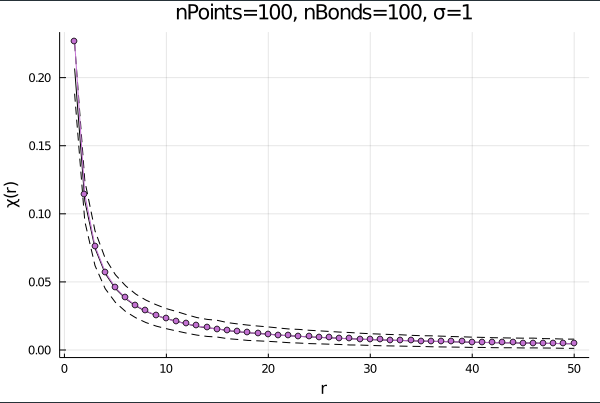
\includegraphics[width=0.8\textwidth]{figures/correlationFunction.png}
	\caption{The average correlation function (black) $\xi(r)$ and its standard deviation (dashed lines) of  1000 realizations of a connectivity graph with $N=100, nBonds=100, \sigma=1$. In pink, dotted, the fit of the average correlation function to the curve $y = (4.5 r + 0.5) ^ {-1} $.} 
	\label{fig:correlationFunction}
\end{figure}

Using these algorithms, we first study the number of clusters for different configurations of the system.
Figure \ref{fig:nClusters} shows the average number of clusters as a function of the number of bonds, fixing the total number of modes, $N=1000$ and the $\sigma=2$.

\begin{figure}[t]
	\centering
	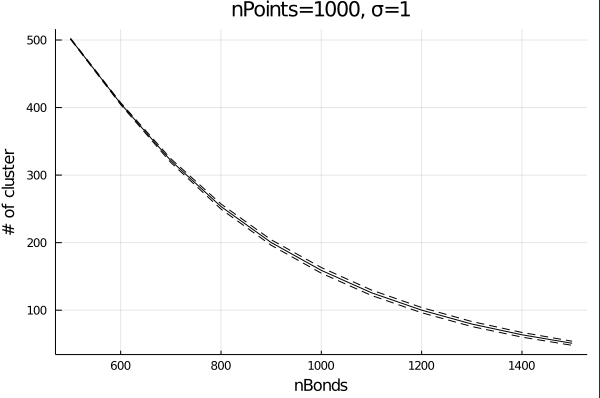
\includegraphics[width=0.8\textwidth]{figures/nClusters.png}
	\caption{Average number of clusters and standard deviation as a function of number of bonds, for fixed number of nodes and $\sigma$. }
	\label{fig:nClusters}
\end{figure}

We also show in figures  the distribution of the lengths of the clusters for fixed number of nodes but varying number of bonds and  $\sigma.$ Here we see how a small number of bonds leads to (as one would expect) all clusters being of length 1 (i.e. a very disconnected graph). The distribution skews towards higher cluster sizes with higher number of modes, and finally for a high enough (nBonds=200) number of bonds almost all nodes are connected.

\begin{figure}
		\centering
		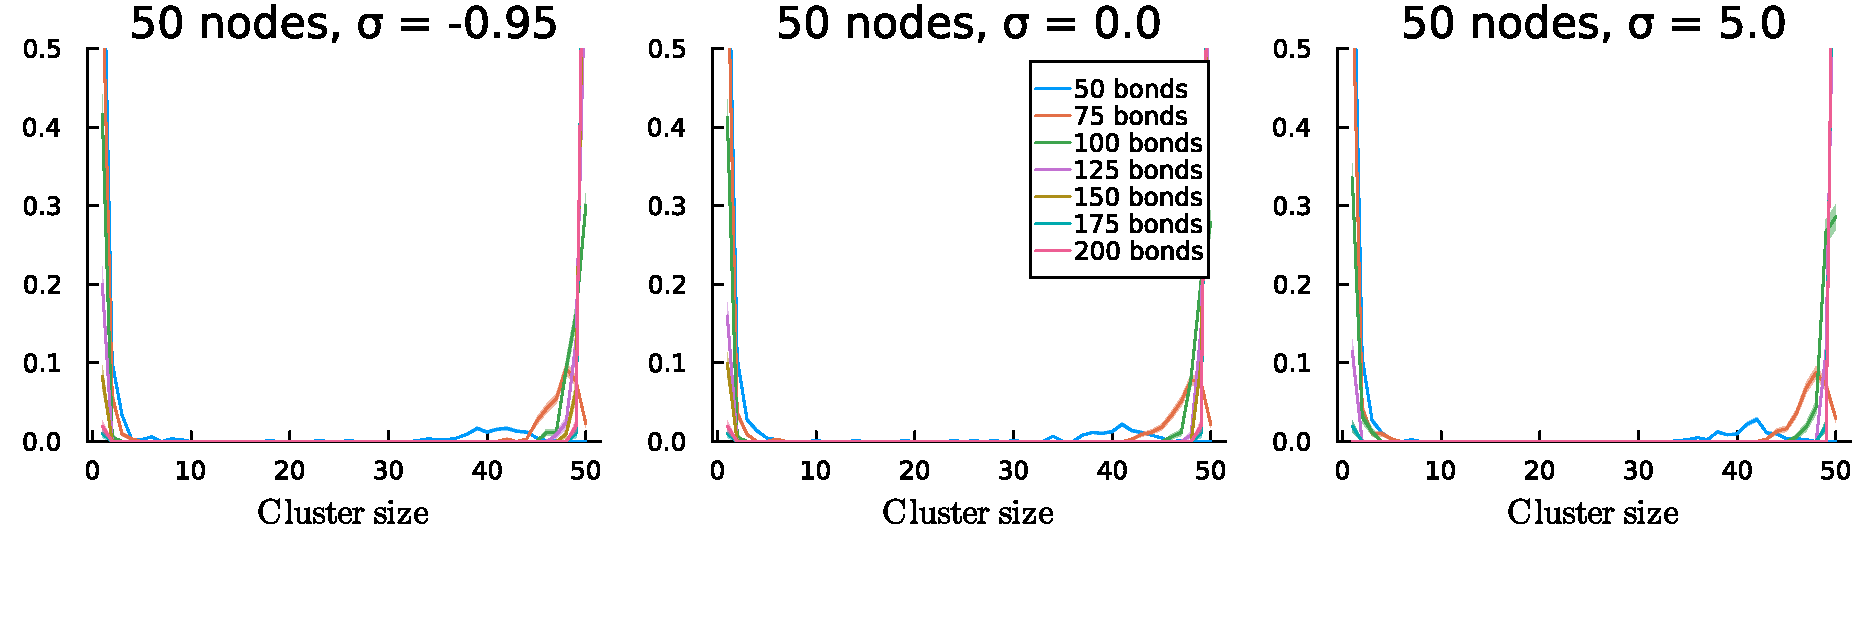
\includegraphics[width=\textwidth]{figures/clusterSizeDistribution.pdf}
	\caption{Normalized distributions of cluster sizes for fixed number of nodes $N=50$ and  varying $\sigma$ values, as indicated at the top of each panel, for different number of bonds among the nodes, as indicated in the legend of the middle panel.}
	\label{fig:clusterLengthDistributionsigma2}
\end{figure}


\begin{figure}
\begin{subfigure}{0.32\textwidth}
		\centering
		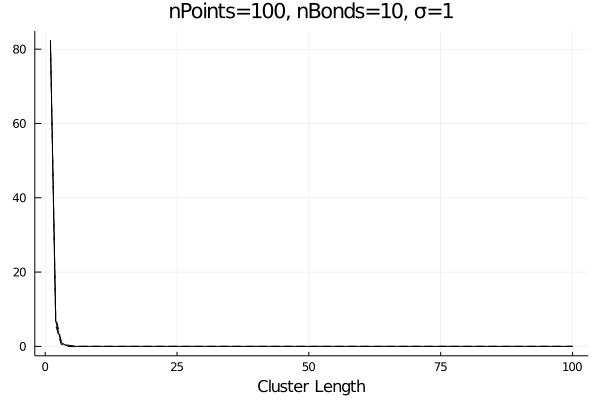
\includegraphics[width=\textwidth]{figures/ClusterLengthDistributionWithNBonds/sigma1/clusterLengthDistribution_nPoints100 nBonds10 sigma1.png}
	\end{subfigure}
\hspace{-0.2cm}
\begin{subfigure}{0.32\textwidth}
		\centering
		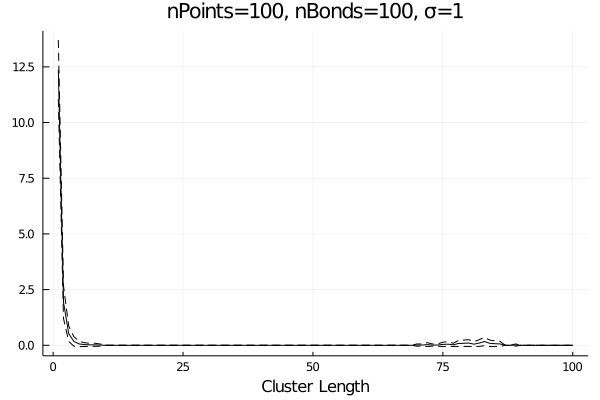
\includegraphics[width=\textwidth]{figures/ClusterLengthDistributionWithNBonds/sigma1/clusterLengthDistribution_nPoints100 nBonds100 sigma1.png}
\end{subfigure} \hspace{-0.3cm}
\begin{subfigure}{0.32\textwidth}
		\centering
		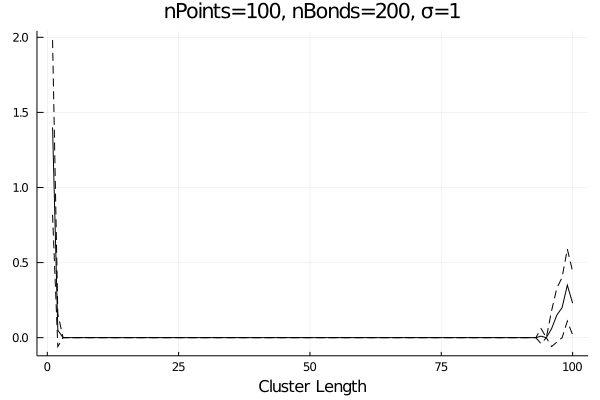
\includegraphics[width=\textwidth]{figures/ClusterLengthDistributionWithNBonds/sigma1/clusterLengthDistribution_nPoints100 nBonds200 sigma1.png}
	\end{subfigure}
	\caption{The distribution of the cluster Length for fixed number of nodes $N=100$ and  $\sigma=1$, for different number of bonds among the nodes. The panels are arranged as in the figure \ref{fig:clusterLengthDistributionsigma2}}
	\label{fig:clusterLengthDistributionsigma1}
\end{figure}

\begin{figure}
\begin{subfigure}{0.32\textwidth}
		\centering
		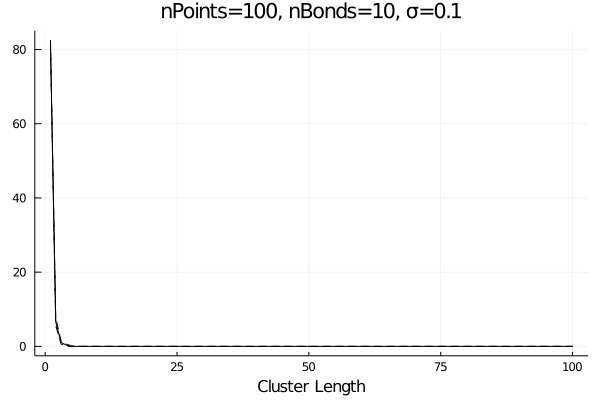
\includegraphics[width=\textwidth]{figures/ClusterLengthDistributionWithNBonds/sigma0.1/clusterLengthDistribution_nPoints100 nBonds10 sigma0.1.png}
	\end{subfigure}
\hspace{-0.2cm}
\begin{subfigure}{0.32\textwidth}
		\centering
		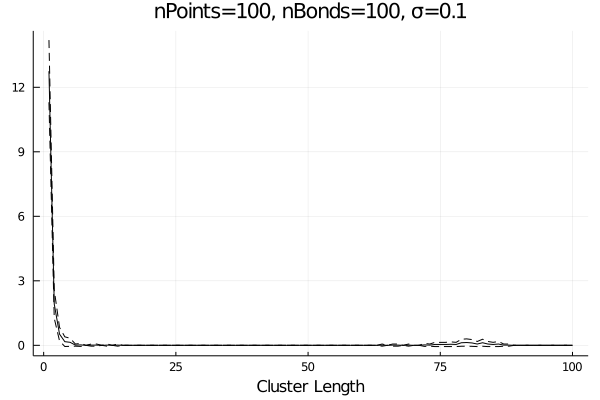
\includegraphics[width=\textwidth]{figures/ClusterLengthDistributionWithNBonds/sigma0.1/clusterLengthDistribution_nPoints100 nBonds100 sigma0.1.png}
\end{subfigure} \hspace{-0.3cm}
\begin{subfigure}{0.32\textwidth}
		\centering
		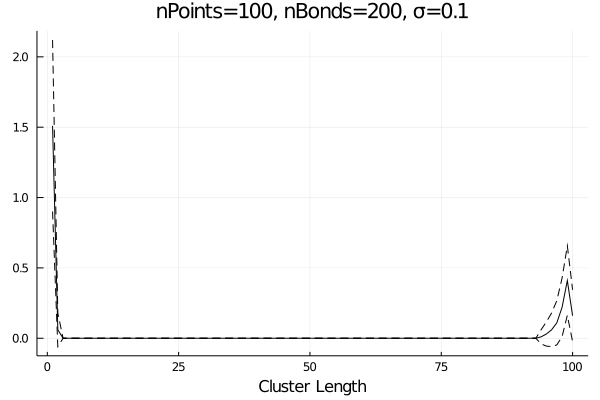
\includegraphics[width=\textwidth]{figures/ClusterLengthDistributionWithNBonds/sigma0.1/clusterLengthDistribution_nPoints100 nBonds200 sigma0.1.png}
	\end{subfigure}
	\caption{The distribution of the cluster Length for fixed number of nodes $N=100$ and  $\sigma=0.1$, for different number of bonds among the nodes. The panels are arranged as in the figure \ref{fig:clusterLengthDistributionsigma2}.}
	\label{fig:clusterLengthDistributionsigma0.1}
\end{figure}

